\hypertarget{what-determines-the-value}{%
\section{What determines the value}\label{what-determines-the-value}}

Section 4 concerned the form of the constant slot and Section 5 the
range of values compatible with records. This section asks what a
model's own dynamics and records determine about the value. We use a
small self-consistent lattice model in which a background offset plays
the role of the constant term, classify its orbits exactly, and then ask
which readouts recover the offset. A closed-ledger extension of the
model shows how the price construction of Section 4 turns the absolute
value into a gauge coordinate.

\hypertarget{the-lattice-model}{%
\subsection{The lattice model}\label{the-lattice-model}}

The model comes from the Six Birds corpus; its source files were copied
into this repository with a hash manifest, re-run, and re-classified by
independently written code with exact agreement on every row (Appendix
C). A complex field \(\psi\) on an eight-site ring sources the potential
it moves in:

\[T_{00,i}[\psi]=|(\nabla\psi)_i|^2+V_{{\rm bg},i}\,|\psi_i|^2,\qquad V_i[\psi]=V_{{\rm bg},i}+\kappa\,T_{00,i}[\psi].\]

One update takes the normalized lowest eigenvector \(\phi\) of
\(H=K+\operatorname{diag}(V[\psi])\), where \(K\) is the ring's kinetic
operator, replaces it by \(\phi\,e^{-i\arg z}\) with
\(z=\langle\phi,\psi\rangle\) (unless \(|z|\) is below a small
tolerance), and sets \(\psi\leftarrow(\psi+\phi)/\|\psi+\phi\|\) (mixing
\(1/2\)). This is the source's phase convention, which we keep
unchanged. A run is declared converged if, after 60 updates, four
diagnostics are all at most \(10^{-8}\): the size of the last update,
the fixed-point gap between \(\psi\) and the lowest eigenvector of the
final Hamiltonian after the source's phase operation is applied to it
twice, the eigen-equation residual of \(\psi\), and a sourcing residual.
As implemented, the sourcing residual compares the potential with itself
and is identically zero, so in effect three diagnostics are tested. The
background is a fixed site profile plus a scalar offset \(c\). The
original sweep used eighteen offsets in \([-8,10]\) at coupling
\(\kappa=0.3\), and twelve couplings from \(0\) to \(30\) at zero
offset.

The statements below about the original sampled orbits and diagnostics
refer to exact real and complex trajectories on the rational values of
the saved binary inputs: the initial field, the background arrays
(including each shifted array as stored), the couplings and the
thresholds. Decimal labels such as \(\kappa=0.3\) or offset \(-5\) name
those inputs. The statements do not describe trajectories for idealized
decimal inputs or the rounding of each floating-point operation.

The offset is not a symmetry of the dynamics. Shifting the background by
\(c\) changes the potential at site \(i\) by
\[\Delta V_i=c\,\bigl(1+\kappa|\psi_i|^2\bigr),\] which is not constant
across sites unless the density is uniform. Different offsets therefore
give genuinely different self-consistent states, and a readout that kept
the whole state could in principle tell offsets apart.

\hypertarget{finite-budgets-and-limits}{%
\subsection{Finite budgets and
limits}\label{finite-budgets-and-limits}}

In the original sweep, fifteen of the eighteen offsets passed the
60-update test and three, \(\{-5,-3,+10\}\), failed; among the
couplings, \(\kappa\le10\) passed and \(\kappa\in\{15,20,30\}\) failed.
A pass/fail table of this kind is easily read as a map of which
parameter values \emph{admit} a self-consistent state. The exact
analysis shows that it is not.

\begin{theorem}[Orbit classification]\label{thm:orbits}
For the original eight-site model, initial field and mixing $1/2$:
\begin{enumerate}
\item every real background profile and every real coupling admit a positive, normalized, self-consistent ground state;
\item at $\kappa=0.3$, the orbits of all eighteen sampled offsets converge to a self-consistent ground state; fifteen pass
the four-residual test at update 60, and the offsets $-5$, $-3$ and $+10$ fail it there;
\item at zero offset, the orbits for $\kappa\in\{0,0.1,0.3,0.5,1,2,3,5,10\}$ converge and pass the test at update 60; the orbit
for $\kappa=15$ fails the test at every update from 1 to 60, yet converges, entering a certified basin of attraction at
update 178; the orbits for $\kappa=20$ and $\kappa=30$ approach bounded two-cycles, so they have no limit.
\end{enumerate}
\end{theorem}

Each part is mechanized. Part 1 uses Brouwer's fixed-point theorem for
the self-consistency map and does not assume that any iteration
converges; a smooth positive ground branch is also constructed along the
original background for every coupling in \([0,30]\). Parts 2 and 3
follow the exact orbits from the original seed: through finite stretches
by exact arithmetic, and from there by certified contraction into the
limit, or into the attracting two-cycle. All sampled orbits stay
normalized and within the update's legality guards at every step. The
classifications concern the sampled parameter values; they do not cover
every intermediate offset or coupling.

Figure \ref{fig:orbits} shows the same behavior in ordinary floating
point. The three ``failing'' offsets \(-3\), \(+10\) and \(-5\) first
pass the diagnostics at updates 74, 86 and 105, the coupling
\(\kappa=15\) at update 176, and the couplings \(20\) and \(30\) settle
into oscillations whose residuals stay of order one. The 60-update test
therefore measures how fast an orbit converges, not whether a
self-consistent state exists. Nor does it separate the offset from the
coupling as kinds of parameter: both have sampled values that fail at 60
updates and converge later. The coupling differs only in having sampled
values, \(20\) and \(30\), whose orbits have no limit even though
self-consistent states exist there.

\begin{figure}[t]
\centering
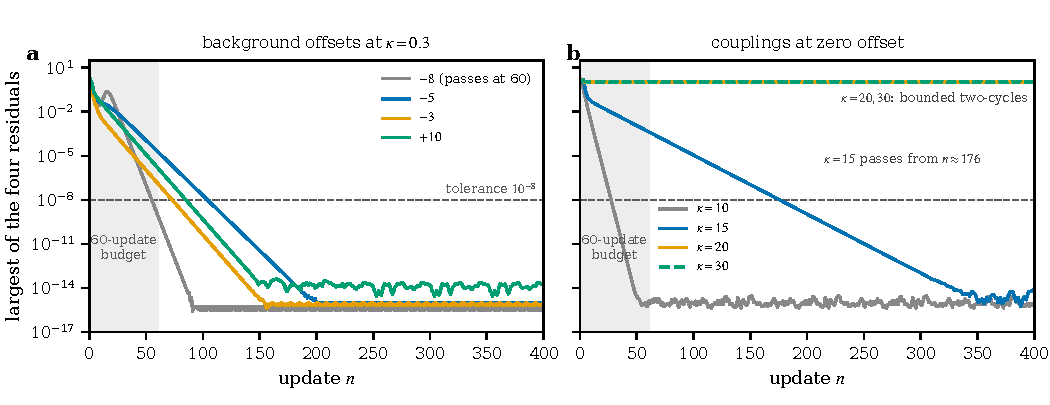
\includegraphics[width=\textwidth]{F4_orbits.pdf}
\caption{\textbf{Finite budget versus limit in the lattice model.} Largest of the four convergence residuals after $n$
updates, computed in floating point with the unchanged original code. \emph{Left:} offsets $-5$, $-3$ and $+10$ fail the
test at the 60-update budget (shaded) but pass it later; offset $-8$ is shown for comparison. \emph{Right:} coupling
$\kappa=15$ first passes at update 176; $\kappa=20$ and $30$ approach bounded two-cycles. The exact statements, including
convergence, are in \Cref{thm:orbits}.}
\label{fig:orbits}
\end{figure}

\hypertarget{readouts-that-do-not-determine-the-offset}{%
\subsection{Readouts that do not determine the
offset}\label{readouts-that-do-not-determine-the-offset}}

Two Boolean readouts are natural for this model: whether the
four-residual test passes at update 60, and whether the orbit has a
limit at all.

\begin{corollary}[Readout nonidentifiability]\label{thm:readout}
Let $r_{60}(c)$ be the outcome of the four-residual test at update 60 and $r_\infty(c)$ the truth value of
"the orbit has a limit", for the eighteen sampled offsets $c$ at $\kappa=0.3$. No function
$\phi:\{\mathrm{true},\mathrm{false}\}\to\mathbb Q$ satisfies $\phi(r_{60}(c))=c$ for all eighteen offsets, and none satisfies
$\phi(r_\infty(c))=c$. Concretely, $r_{60}(-8)=r_{60}(-2)=\mathrm{true}$, and $r_\infty$ is true for every offset.
\end{corollary}

Given \Cref{thm:orbits}, the corollary is elementary, and it is
mechanized with the readouts defined from the actual orbit propositions
rather than from a table. Its content is the precise sense in which the
offset is a \emph{contingent modulus} of this model: the two convergence
readouts leave it undetermined, so it must be supplied as input or
chosen by some further rule. Three limits of the statement matter. The
finite readout does distinguish passing from failing offsets. A richer
readout, such as the full converged state, could recover the offset,
since the dynamics depend on it. And nothing here excludes an additional
selection rule.

\hypertarget{a-closed-ledger-makes-the-absolute-value-a-gauge-coordinate}{%
\subsection{A closed ledger makes the absolute value a gauge
coordinate}\label{a-closed-ledger-makes-the-absolute-value-a-gauge-coordinate}}

The offset in the lattice model is visible to the full state because it
couples to the density through \(\kappa\). Section 4 suggests what would
hide it: a global budget whose price absorbs a common shift. The
sitewise shift \(c\,(1+\kappa\rho_i)\), with \(\rho_i=|\psi_i|^2\), is
exactly the derivative with respect to \(\rho_i\) of \(c\,Q_\kappa\),
where
\[Q_\kappa(\psi)=\sum_i\Bigl(\rho_i+\tfrac{\kappa}{2}\rho_i^2\Bigr),\]
and among quadratic ledgers \(a\rho+b\rho^2\) this one is forced. The
added force \(c\,(1+\kappa\rho_i)\psi_i\) is therefore normal to the
level sets of \(Q_\kappa\). Fixing \(Q_\kappa\) adds a constraint to the
model, with a multiplier \(\mu\). The compensated potential
\[V_i^{\rm closed}=V_{{\rm bg},i}+\kappa T_{00,i}-\mu\,(1+\kappa\rho_i)=(V_{{\rm bg},i}-\mu)(1+\kappa\rho_i)+\kappa\,|(\nabla\psi)_i|^2\]
depends on the background only through \(V_{\rm bg}-\mu\), so it is
unchanged under \((V_{\rm bg},\mu)\mapsto(V_{\rm bg}+c,\mu+c)\) for
every field. A presentation of the closed model is a triple (state,
background, price); its invariant record keeps the full state and every
relative background coordinate \(V_{{\rm bg},i}-\mu\).

\begin{theorem}[Gauge modulus]\label{thm:gauge}
In the ledger-closed model:
\begin{enumerate}
\item two presentations have the same invariant record if and only if they differ by a common shift of background and price;
\item the absolute price, equivalently the absolute background, is not a function of the invariant record; in the
allocation form of the closed model this holds already on an explicit pair of two-site optimality certificates, with
$\kappa=2$, densities $(1/2,1)$, ledger budget $11/4$ and positive prices $3/2$ and $5/2$;
\item no selector depending only on the invariant record transforms correctly under the joint shift
$(V_{\rm bg},\mu)\mapsto(V_{\rm bg}+c,\mu+c)$, since the shift leaves the record unchanged while an absolute value would
have to move by $c$;
\item any linear projection that annihilates the ledger normal makes the projected force at a given state invariant under
the common shift; and in the allocation form of the closed model, two projected-gradient histories with the same initial state, budget, step size and
coefficients, whose backgrounds differ by a common shift, coincide at every step.
\end{enumerate}
In addition, no probability measure on the line of absolute values is invariant under all real translations.
\end{theorem}

Parts 1 to 4 are mechanized as stated. Invariance of the continuous-time
constrained flow under the shift follows from part 4 together with the
existence and uniqueness argument below, and is not mechanized. The
final statement is the standard argument that translation-invariance
would give every unit interval the same mass, which is impossible for a
probability measure; it is not mechanized. The extension changes the
model: it adds the ledger and replaces the damped eigenvector update by
a constrained flow, with the normalization and \(I=\sum_i\rho_i^2\) held
fixed, that keeps the original local force. That the projection onto
this constraint set is well defined and the flow exists globally is a
paper-level argument, not mechanized: for \(\kappa>0\), on the level set
\(\sum_i\rho_i=1\), \(I=17/108\), which is nonempty and compact, the two
constraint normals are independent (because \(I\ne1/m\) for
\(m=1,\ldots,8\)), so the projected field is smooth and tangent, and
solutions exist and are unique for all times.

The theorem gives a sharper sense to the title in this model. The
absolute value is not merely unread by a coarse test; it is a gauge
coordinate of the closed description. A convention such as \(\mu=0\), or
any rule that picks a value for outside reasons, remains available. What
is excluded is recovering the value from the invariant layer itself, and
assigning it a translation-invariant probability. Any prior over the
absolute value therefore has to carry symmetry-breaking content, a point
that returns in Section 7. Nothing here shows that the physical
cosmological constant is a gauge coordinate of any physical theory.

\hypertarget{two-descriptions-and-a-mediator}{%
\subsection{Two descriptions and a
mediator}\label{two-descriptions-and-a-mediator}}

The headline form of the cosmological-constant problem compares a
vacuum-energy estimate made in quantum field theory with a constant
measured through gravity. In the Six Birds corpus this comparison is
framed as one between two coarse descriptions of a common finer system.
A finite version of that framing has a precise theorem, which we record
because it states what any common description would have to retain.

Let \(H=\{0,1\}^4\) with coordinates \((d_0,d_1,d_2,d_3)\), and consider
the two readouts \(q_Q(d)=(d_0,d_1,d_2)\) and \(q_G(d)=(d_0,d_2,d_3)\).
Neither determines the other.

\begin{theorem}[Mediator]\label{thm:mediator}
A deterministic map $r$ on $H$, with any codomain, determines both $q_Q$ and $q_G$ if and only if it determines the full
state $d$, which holds if and only if $r$ is injective. In particular such a mediator has exactly sixteen distinct records.
\end{theorem}

The theorem is mechanized, and the recovery map is explicit: three
coordinates from the first decoder and the fourth from the second. It
concerns information, not storage: it does not require four separate
fields or four dimensions. The companion question, whether the two
fill-in rules commute, has an affirmative answer for the original model:
the completions given by uniform conditional means over the two readouts
commute on every observable. A separately declared weighted example does
not commute: on a three-cell block with cell weights \(5\), \(1\) and
\(3\), applying the two conditional means in opposite orders to the
observable \((0,1,0)\) gives values that differ by \(1/16\) on the first
cell.

For the cosmological-constant problem the lesson is limited and
structural. Comparing a number computed in one description with a
parameter of another requires a map between them, and in this finite
model any map that supports both readouts must retain everything either
one sees. The theorem does not identify the two readouts with quantum
field theory and gravity, does not compute a vacuum-energy discrepancy,
and does not resolve the cosmological-constant problem.
